% % % % % % % % % % % % % % % % % % % % % % % % % % % % % % % % % %
%  Devolutiva — Fase 1: Imersão
%  Disciplina: Design Thinking (DE_233) — ETE Cícero Dias
%  Profa. Samara Silva  ·  Recife, 28 de junho de 2026
% % % % % % % % % % % % % % % % % % % % % % % % % % % % % % % % % %

\documentclass[
  sigconf,
  nonacm, % Remove o rodapé da ACM
  language=portuguese
]{acmart}

% ── Desliga rodapé ACM ──────────────────────────────────────
\settopmatter{printacmref=false}
\setcopyright{none}
\acmYear{2026}
\let\balance\relax

% ── Mata a página temporária da ACM (compilação única via API) ──
\makeatletter
\def\acm@addtemp@page{}
\makeatother

% ── Pacotes ─────────────────────────────────────────────────
\usepackage[portuguese]{babel}
\usepackage{microtype}
\usepackage{booktabs}
\usepackage{tabularx}
\usepackage{array}
\usepackage{colortbl}
\usepackage[dvipsnames,table]{xcolor}
\usepackage[inline]{enumitem}
\usepackage{graphicx}
\usepackage{adjustbox}
\usepackage{fancyhdr}
\usepackage{eso-pic} % Para a capa preencher toda a página sem gerar páginas em branco

% ── Ajuste contra quebras de texto ruins (Textos Cortados) ──
\tolerance=1000
\emergencystretch=1.5em

% ── Cores ───────────────────────────────────────────────────
\definecolor{cgood}{HTML}{1E6B3A}
\definecolor{cwarn}{HTML}{8B4500}
\definecolor{cred}{HTML}{C0392B}
\definecolor{cmuted}{HTML}{666666}
\definecolor{crow}{HTML}{F2EFEB}

% ── Colunas customizadas para tabela ────────────────────────
\newcolumntype{L}[1]{>{\raggedright\arraybackslash}p{#1}}
\newcolumntype{C}[1]{>{\centering\arraybackslash}p{#1}}

% ── Comando nota destacada ───────────────────────────────────
\newcommand{\notadestaque}[2]{%
  \noindent\textbf{Nota:}\enspace%
  {\large\bfseries\color{cred}#1\,/\,#2\,pts}%
}

% ── Comando label de status ──────────────────────────────────
\newcommand{\statusok}[1]{{\small\bfseries\color{cgood}#1}}
\newcommand{\statuswarn}[1]{{\small\bfseries\color{cwarn}#1}}

% ── Renomeações PT-BR ────────────────────────────────────────
\AtBeginDocument{%
  \renewcommand{\abstractname}{Resumo}
  \renewcommand{\figurename}{Figura}
  \renewcommand{\tablename}{Tabela}
}

% ────────────────────────────────────────────────────────────
\begin{document}

% ── CAPA ────────────────────────────────────────────────────
\thispagestyle{empty}
\AddToShipoutPictureBG*{%
  \AtPageLowerLeft{%
    \IfFileExists{capa.png}{%
      
\includegraphics[width=\paperwidth,height=\paperheight]{capa.png}%
    }{%
      \IfFileExists{../../capa.png}{%
        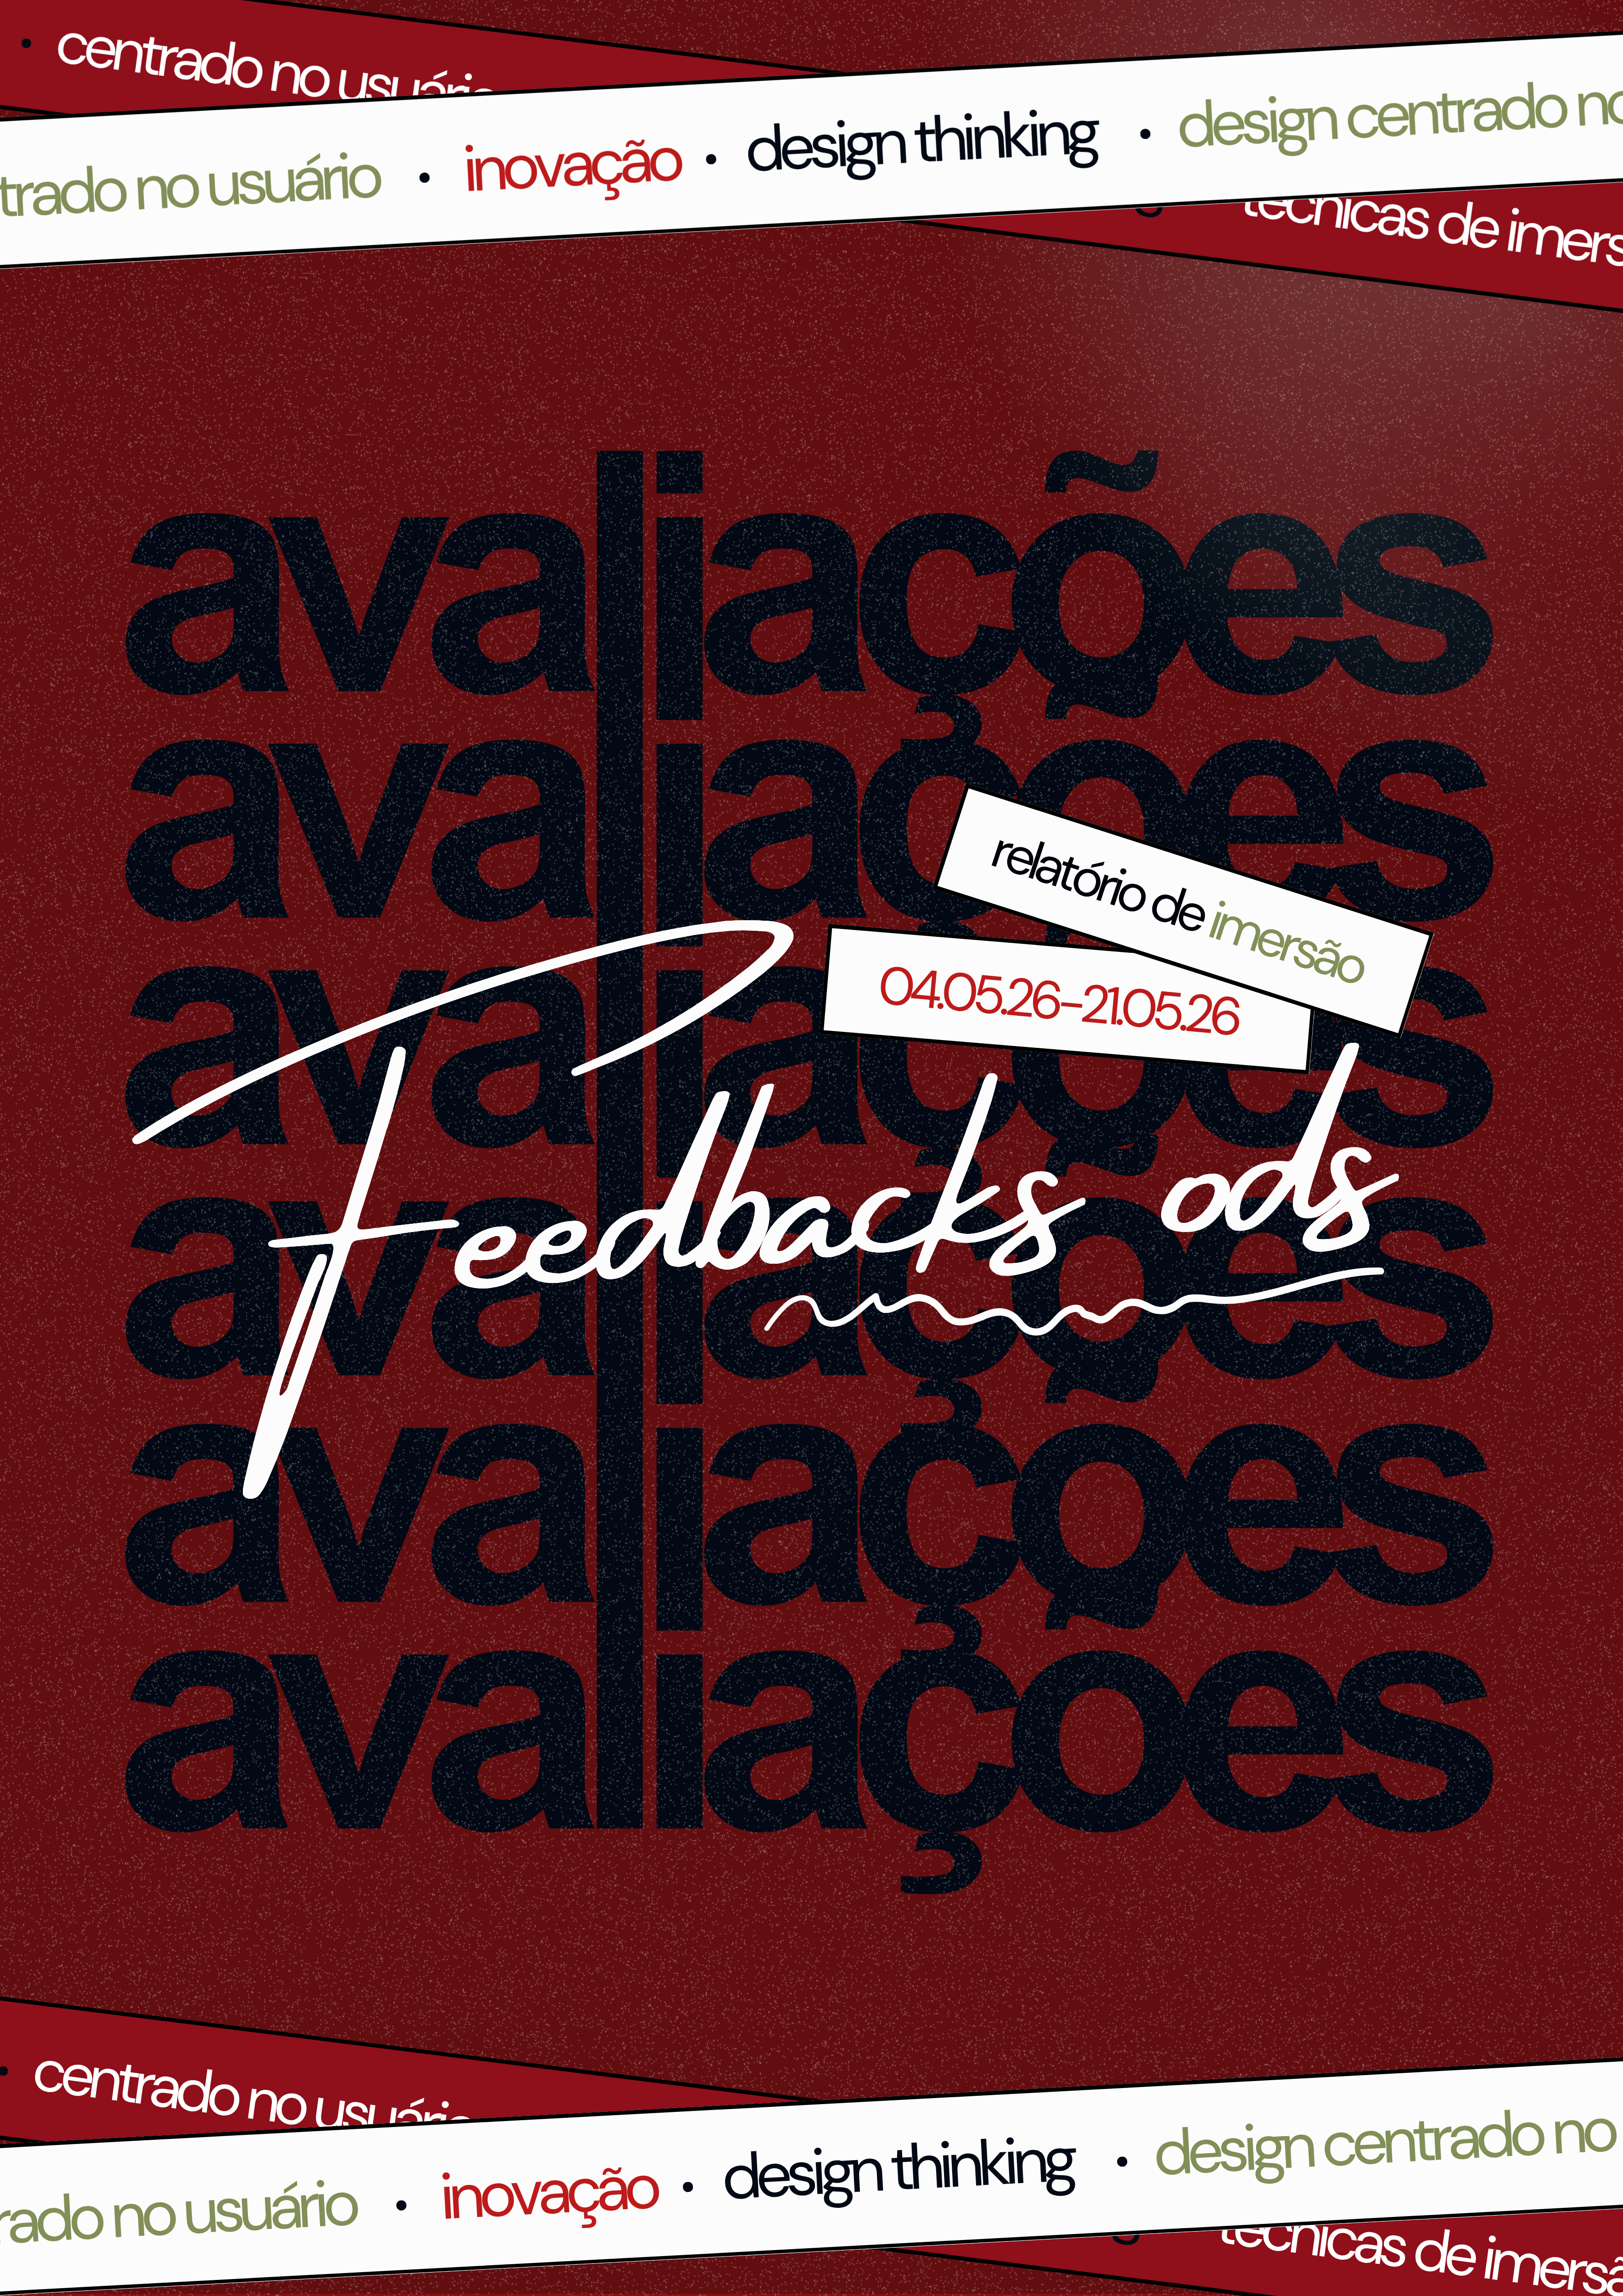
\includegraphics[width=\paperwidth,height=\paperheight]{../../capa.png}%
      }{%
        \parbox[b][\paperheight]{\paperwidth}{%
          \vspace*{10cm}\begin{center}{\large\color{gray}[capa.png não encontrada]}\end{center}%
        }%
      }%
    }%
  }%
}
\mbox{} % Caixa vazia para garantir que a página da capa seja gerada e preenchida
\clearpage

% ── CONFIGURAÇÃO DE PÁGINA PÓS-CAPA ─────────────────────────
\setcounter{page}{1}
\pagestyle{fancy}
\fancyhf{}
\renewcommand{\headrulewidth}{0pt}
\fancyfoot[C]{\thepage}
\setlength{\headsep}{0.8cm} % Distancia o cabeçalho do conteúdo das colunas

% ── METADADOS ────────────────────────────────────────────────
\title{Feedback Avaliativo de Projeto: Design Thinking --- Avaliação Completa}

\author{Profa.\ Samara Silva}
\authornote{Grupo: \textbf{Grupo 03 - Doação de Alimentos} \textperiodcentered\ Per\'{i}odo: 22 de maio de 2026 \textperiodcentered\ Avaliado em: 28 de junho de 2026.}
\email{samarasilvia.educa@gmail.com}
\affiliation{%
  \institution{ETE C\'{i}cero Dias}
  \department{M\'{o}dulo 1 --- Turma A · 2026.1}
  \city{Recife}
  \state{Pernambuco}
  \country{Brasil}
}

\author{Grupo 03 - Doação de Alimentos}
\affiliation{%
  \institution{ETE C\'{i}cero Dias}
  \department{Turma --- Turma A · 2026.1}
  \city{Recife}
  \state{Pernambuco}
  \country{Brasil}
}
\maketitle

\vspace{1em}
\section{Avaliação — Design Thinking}

\notadestaque{7,64}{11,00}

A seguir o detalhamento por fase da disciplina.

\subsection{Fase 1 — Imersão}

\notadestaque{1,39}{3,00}

\subsubsection*{Resumo dos Critérios}

\rowcolors{2}{crow}{white}
\begin{tabular}{@{} L{2.6cm} C{2.5cm} C{1.1cm} C{1.1cm} @{}}
\toprule
\textbf{Critério} & \textbf{Status} & \textbf{Nota} & \textbf{Máx.} \\
\midrule
Pesquisa Desk & \statuswarn{Completo c/ ressalvas} & \textbf{0,42} & 0,50 \\
Matriz de Alinhamento & \statuswarn{Faltou pouco c/ erros} & \textbf{0,30} & 0,50 \\
Matriz CSD \& Perguntas de pesquisa & \statuswarn{Completo c/ ressalvas} & \textbf{0,42} & 0,50 \\
Pesquisa Primária & \statuswarn{Faltou muito e errou} & \textbf{0,25} & 1,50 \\
\midrule
\textbf{Total} & & \textbf{\color{cred}1,39} & \textbf{3,00} \\
\bottomrule
\end{tabular}

\subsubsection*{Comentários}

\subsection{Pesquisa Desk}

\noindent\statuswarn{0,42\,/\,0,50 pts · Completo c/ ressalvas}

\begin{itemize}[leftmargin=14pt,itemsep=1pt,topsep=3pt,parsep=0pt]
  \item[\textcolor{cgood}{$\checkmark$}] {\small\textcolor{cgood}{Dados secundários relevantes e atuais sobre o ODS escolhido}}
  \item[\textcolor{cgood}{$\checkmark$}] {\small\textcolor{cgood}{Fontes confiáveis: ONU, IBGE, artigos acadêmicos ou jornalísticos}}
  \item[\textcolor{cgood}{$\checkmark$}] {\small\textcolor{cgood}{Contextualiza o problema com base factual}}
  \item[\textcolor{cgood}{$\checkmark$}] {\small\textcolor{cgood}{Conexão clara entre os dados e o problema}}
  \item[$\square$] {\small\textcolor{cmuted}{Coerência entre a CSD e o que foi pesquisado}}
  \item[\textcolor{cgood}{$\checkmark$}] {\small\textcolor{cgood}{Mínimo de 5 referências/links, esperado 8, ideal de 15 para cima}}
\end{itemize}

Outro ponto que merece atenção é a coerência entre a Matriz CSD e as pesquisas realizadas durante a etapa de imersão. Conforme evidenciado pela ausência de atendimento a esse critério, não foi possível identificar uma conexão clara entre parte das dúvidas levantadas na CSD e os dados posteriormente coletados.

A matriz apresenta perguntas e dúvidas bastante pertinentes e estratégicas, demonstrando uma boa reflexão inicial sobre o problema. No entanto, muitas dessas questões não foram contempladas na pesquisa secundária (artigos, notícias, relatórios, sites e demais fontes consultadas), o que gera uma lacuna entre o que o grupo declarou precisar descobrir e aquilo que efetivamente investigou.

Também não foi possível verificar se essas dúvidas foram respondidas por meio da pesquisa de campo. Considerando a quantidade reduzida de perguntas presentes no formulário, há indícios de que parte significativa das questões levantadas na CSD permaneceu sem validação.

É importante lembrar que a Matriz CSD não deve ser tratada apenas como uma atividade isolada. As dúvidas registradas nela devem orientar as etapas seguintes da pesquisa, servindo como direcionadoras da investigação. Ao final da imersão, espera-se que a maior parte dessas dúvidas tenha sido respondida, validada ou refutada por meio das evidências coletadas.

Como sugestão de melhoria, recomenda-se revisar as dúvidas levantadas na CSD e verificar, para cada uma delas, qual fonte de pesquisa foi utilizada para respondê-la e quais evidências foram encontradas. Esse exercício contribui para fortalecer o rigor metodológico e a rastreabilidade das decisões tomadas ao longo do projeto.

\subsection{Matriz de Alinhamento}

\noindent\statuswarn{0,30\,/\,0,50 pts · Faltou pouco c/ erros}

\begin{itemize}[leftmargin=14pt,itemsep=1pt,topsep=3pt,parsep=0pt]
  \item[\textcolor{cgood}{$\checkmark$}] {\small\textcolor{cgood}{Identifica claramente quem é afetado pelo problema}}
  \item[\textcolor{cgood}{$\checkmark$}] {\small\textcolor{cgood}{Define o que o grupo pretende descobrir durante a imersão}}
  \item[\textcolor{cgood}{$\checkmark$}] {\small\textcolor{cgood}{As técnicas de imersão escolhidas são coerentes com os objetivos da pesquisa}}
  \item[\textcolor{cgood}{$\checkmark$}] {\small\textcolor{cgood}{Delimita adequadamente o que está dentro do escopo do projeto}}
  \item[$\square$] {\small\textcolor{cmuted}{Delimita adequadamente o que está fora do escopo do projeto}}
  \item[\textcolor{cgood}{$\checkmark$}] {\small\textcolor{cgood}{Apresenta uma hipótese inicial de solução relacionada ao problema investigado}}
  \item[$\square$] {\small\textcolor{cmuted}{Os resultados esperados da imersão são claros e coerentes com os objetivos da pesquisa}}
  \item[\textcolor{cgood}{$\checkmark$}] {\small\textcolor{cgood}{Há coerência entre os diferentes campos da matriz (problema, público, escopo, pesquisa e solução)}}
  \item[\textcolor{cgood}{$\checkmark$}] {\small\textcolor{cgood}{Preenchida com respostas, impressões ou perguntas reais do grupo sobre o problema}}
  \item[$\square$] {\small\textcolor{cmuted}{Linguagem clara e coerente, facilitando a compreensão das intenções do grupo}}
  \item[\textcolor{cgood}{$\checkmark$}] {\small\textcolor{cgood}{Serviu de base para planejar a pesquisa primária}}
\end{itemize}

A matriz de alinhamento apresenta algumas inconsistências que precisam ser ajustadas. Em particular, observei que a linguagem em algumas partes está no tempo verbal incorreto, o que acabou dificultando a interpretação do conteúdo.

Por exemplo:

\begin{itemize}[leftmargin=14pt,itemsep=2pt,topsep=4pt]
  \item "Algumas pessoas já têm" → presente do indicativo 
  \item "outras que ainda não doaram" → pretérito perfeito 
  \item "também têm interesse" → presente do indicativo 
  \item "falta direcionamento" → presente do indicativo 
\end{itemize}

Embora esse ponto não seja crítico, ele compromete a uniformidade e a clareza da matriz, o que comprometeu a minha interpretação. Recomenda-se que a seção “O que o grupo quer descobrir?” esteja sempre no \textbf{presente}, refletindo a situação atual, e seja apresentada de forma direta ou narrativa, sem misturar tempos verbais ou repetir ideias.

Sugestões de formulação:

\begin{enumerate}[leftmargin=14pt,itemsep=2pt,topsep=4pt]
  \item \textbf{Versão em tópicos (direta):}
\end{enumerate}

\begin{itemize}[leftmargin=14pt,itemsep=2pt,topsep=4pt]
  \item O costume das pessoas em doar alimentos.
  \item O interesse de pessoas que ainda não doaram em realizar doações.
  \item Se existe direcionamento sobre como e onde realizar doações.
\end{itemize}

\begin{enumerate}[leftmargin=14pt,itemsep=2pt,topsep=4pt]
  \item \textbf{Versão narrativa (fluida):}
\end{enumerate}

\begin{itemize}[leftmargin=14pt,itemsep=2pt,topsep=4pt]
  \item “Queremos descobrir se as pessoas têm o costume de doar alimentos, se aquelas que ainda não doaram possuem interesse em doar, e se existe direcionamento sobre como e onde realizar essas doações.”
\end{itemize}

Outro ponto relevante refere-se ao tópico \textbf{“O que está fora do escopo”}, que não foi preenchido. Este campo deve indicar aspectos que estão além do controle do grupo, como políticas públicas, ações governamentais ou legislações. Por exemplo, iniciativas para fomentar doações de alimentos ou leis específicas do país. É fundamental que essa seção seja preenchida, pois não pode permanecer em branco.

Quanto ao \textbf{“Resultado esperado da imersão”}, observei que há uma interpretação incorreta. O objetivo da imersão não é resolver o problema diretamente por meio de pesquisas passivas, mas sim aprofundar o conhecimento sobre o contexto, coletar dados e entender o panorama do problema. Portanto, este tópico deve indicar o que se espera compreender, como esclarecer dúvidas e identificar limites e padrões da questão investigada.

Também é importante evitar a repetição ao expressar o problema da doação de alimentos e seu desperdício. A clareza na formulação do problema contribui para uma análise mais consistente e estratégica.

Por fim, em relação ao público afetado, sugiro refletir se ele está completamente mapeado. Limitar-se apenas a pessoas em situação de rua ou com menor condição financeira pode não contemplar todos os impactos do problema. Famílias de classe média, por exemplo, também podem ser afetadas e merecem ser consideradas no estudo.

\subsection{Matriz CSD \& Perguntas de pesquisa}

\noindent\statuswarn{0,42\,/\,0,50 pts · Completo c/ ressalvas}

\begin{itemize}[leftmargin=14pt,itemsep=1pt,topsep=3pt,parsep=0pt]
  \item[\textcolor{cgood}{$\checkmark$}] {\small\textcolor{cgood}{Os três quadrantes preenchidos: Certezas, Suposições, Dúvidas}}
  \item[\textcolor{cgood}{$\checkmark$}] {\small\textcolor{cgood}{Reflete o que o grupo sabe e precisa descobrir sobre o problema e seu contexto}}
  \item[\textcolor{cgood}{$\checkmark$}] {\small\textcolor{cgood}{Conteúdo específico do projeto — não genérico}}
  \item[\textcolor{cgood}{$\checkmark$}] {\small\textcolor{cgood}{Revela pensamento crítico}}
  \item[\textcolor{cgood}{$\checkmark$}] {\small\textcolor{cgood}{O quadrante de CERTEZAS expõe informações comprovadas ou confirmadas sobre o problema}}
  \item[\textcolor{cgood}{$\checkmark$}] {\small\textcolor{cgood}{Os itens do quadrante de CERTEZA estão relacionados diretamente ao contexto e ao público afetado}}
  \item[\textcolor{cgood}{$\checkmark$}] {\small\textcolor{cgood}{O quadrante de SUPOSIÇÕES expõe Informações que o grupo acha que são verdadeiras, mas ainda não comprovou}}
  \item[\textcolor{cgood}{$\checkmark$}] {\small\textcolor{cgood}{Os itens do quadrante de SUPOSIÇÃO demonstram reflexão sobre possíveis causas, comportamentos ou necessidades}}
  \item[\textcolor{cgood}{$\checkmark$}] {\small\textcolor{cgood}{O quadrante de DÚVIDAS expõem perguntas que o grupo precisa responder na pesquisa ou imersão como um todo}}
  \item[\textcolor{cgood}{$\checkmark$}] {\small\textcolor{cgood}{Os itens do quadrante de DÚVIDAS representam lacunas reais de conhecimento}}
  \item[$\square$] {\small\textcolor{cmuted}{O conteúdo da matriz está focado no problema investigado e não apenas no tema ou na ODS}}
  \item[$\square$] {\small\textcolor{cmuted}{Perguntas de Pesquisas formuladas como objetivos que norteiam o projeto geral}}
  \item[$\square$] {\small\textcolor{cmuted}{Deve se ter um mínimo de 5 itens no quadrante de certezas, suposições e dúvidas}}
\end{itemize}

A Matriz CSD foi preenchida de maneira geral correta, demonstrando compreensão da ferramenta. No entanto, identifiquei alguns pontos que precisam de ajustes para garantir que a matriz cumpra plenamente seu propósito dentro da etapa de imersão.

\textbf{Matriz CSD}

\begin{enumerate}[leftmargin=14pt,itemsep=2pt,topsep=4pt]
  \item \textbf{Coluna de Certezas}
\end{enumerate}

Na seção de certezas, foram incluídas informações relacionadas aos Objetivos de Desenvolvimento Sustentável (ODS). Embora o problema esteja conectado às ODS, o foco da CSD deve estar na \textbf{análise e alinhamento do problema} que está sendo investigado, e não nas ODS em si. Certamente, a inclusão pode ter sido feita para atender ao limite de itens da matriz, mas é importante priorizar o contexto do problema, o público-alvo e as condições atuais relacionadas ao tema. Por exemplo, considerar apenas “a doação ajuda pessoas em vulnerabilidade” já é suficiente para essa coluna, desde que bem formulado.

\begin{enumerate}[leftmargin=14pt,itemsep=2pt,topsep=4pt]
  \item \textbf{Coluna de Suposições}
\end{enumerate}

Três itens desta coluna foram preenchidos com foco na solução, o que não é adequado para a etapa de imersão. A etapa atual é voltada para \textbf{entender o problema em profundidade}, identificar hipóteses sobre o contexto e o público, e não propor soluções. As suposições apresentadas, como:

\begin{itemize}[leftmargin=14pt,itemsep=2pt,topsep=4pt]
  \item "O sistema poderá reduzir perdas de alimentos ainda próprios para consumo."
  \item "O sistema pode ajudar a monitorar validade e quantidade dos alimentos."
  \item "O sistema pode aproximar doadores e instituições rapidamente."
\end{itemize}

estão mais relacionadas à \textbf{solução imaginada} pelo grupo do que ao problema investigado.

Na etapa de Imersão, as perguntas principais devem refletir:

\begin{itemize}[leftmargin=14pt,itemsep=2pt,topsep=4pt]
  \item "Qual é o problema?"
  \item "Quem é afetado?"
  \item "Por que isso acontece?"
  \item "Quais necessidades existem?"
  \item "Como as pessoas lidam com isso hoje?"
\end{itemize}

As suposições da CSD deveriam, portanto, propor hipóteses sobre o contexto e o problema, como:

\begin{itemize}[leftmargin=14pt,itemsep=2pt,topsep=4pt]
  \item "Muitas pessoas gostariam de doar alimentos, mas não sabem onde doar."
  \item "Parte dos alimentos é desperdiçada por falta de conexão entre doadores e instituições."
  \item "As instituições têm dificuldade para divulgar suas necessidades."
  \item "Existem pessoas interessadas em receber doações que não sabem onde buscar ajuda."
\end{itemize}

Frases sobre “\textbf{\textit{o sistema poderá…” }}são mais apropriadas para etapas posteriores, como: Ideação, Hipóteses de solução, Proposta de Valor, Canvas da Solução ou Protótipo.

Para evitar essa confusão, recomenda-se criar um \textbf{checkpoint específico}:

\begin{itemize}[leftmargin=14pt,itemsep=2pt,topsep=4pt]
  \item As suposições estão relacionadas ao problema e ao contexto investigado, e não à validação de uma solução.
  \item Evita-se antecipar soluções durante a etapa de imersão.
\end{itemize}

Esse é um erro comum em Design Thinking: os alunos se apaixonam pela ideia da solução logo no início e passam a investigar se ela funciona, quando o foco da imersão deve ser \textbf{verificar se o problema existe da forma imaginada}.

Como avaliadora, não marcaria como “errado”, mas faria a seguinte ressalva:

"As suposições apresentadas concentram-se nos possíveis benefícios da solução proposta. Nesta etapa, recomenda-se formular hipóteses relacionadas ao problema, ao público e ao contexto investigado, deixando a avaliação da solução para as etapas posteriores do processo."

Essa observação está tecnicamente alinhada com a metodologia de Design Thinking e justifica bem uma avaliação do tipo \textbf{“completo com ressalvas”} ou \textbf{“faltou pouco”}, dependendo do restante da entrega.

\begin{enumerate}[leftmargin=14pt,itemsep=2pt,topsep=4pt]
  \item \textbf{Coluna de Dúvidas}
\end{enumerate}

A coluna de Dúvidas está correta e adequada. As questões levantadas são pertinentes e contribuem para direcionar a investigação, não havendo ajustes necessários nesse aspecto. Parabéns ao grupo pelas formulações.

\begin{enumerate}[leftmargin=14pt,itemsep=2pt,topsep=4pt]
  \item \textbf{Formatação}
\end{enumerate}

Vale reforçar a importância de revisar a formatação do Excel para garantir clareza e legibilidade. É essencial que todos os tópicos estejam preenchidos de forma completa e organizada.

\textit{\textbf{Perguntas de Pesquisa}}

Há um desvio metodológico importante na etapa de planejamento das perguntas de pesquisa que precisa ser corrigido: \textbf{houve uma sobreposição entre as Perguntas de Pesquisa e o Roteiro/Formulário do usuário. }Para o rigor acadêmico e prático do Design de Serviços/Produtos, é fundamental distinguir estas três camadas:

\begin{itemize}[leftmargin=14pt,itemsep=2pt,topsep=4pt]
  \item \textbf{Dúvidas (Matriz CSD):} Representam as incertezas internas do grupo. É o levantamento bruto do que a equipe não sabe. ex:\textit{"Os estudantes preferem estudar pelo celular ou pelo notebook?"}
  \item \textit{"Eles ainda têm o costume de usar agenda de papel?"}
  \item \textit{"Quanto tempo eles conseguem focar antes de pegar o celular?"}
\end{itemize}

\begin{itemize}[leftmargin=14pt,itemsep=2pt,topsep=4pt]
  \item \textbf{Perguntas de Pesquisa:} São os objetivos da investigação. Elas guiam o \textit{projeto} e a \textit{equipe}, sintetizando as dúvidas e suposições da CSD em grandes eixos investigativos. \textbf{Essas perguntas não devem ser feitas diretamente ao usuário. }ex:\textit{"Quais são os principais métodos e ferramentas de organização utilizados por universitários hoje, e quais são os maiores gatilhos comportamentais de distração durante o estudo?"}
\end{itemize}

\begin{itemize}[leftmargin=14pt,itemsep=2pt,topsep=4pt]
  \item \textbf{Roteiro/Formulário de Pesquisa:} É o instrumento de coleta. Aqui, as perguntas de pesquisa são traduzidas para a linguagem do usuário, de forma conversacional e empática, para evitar vieses. ex:\textit{"Você poderia me contar como costuma se organizar quando tem uma semana cheia de provas?"}
  \item \textit{"Lembre da última vez que você sentou para estudar e acabou perdendo o foco. Como foi isso? O que acabou tirando a sua atenção?"}
\end{itemize}

\textbf{O impacto desse erro:} Em vez de definirem os eixos estratégicos que o projeto precisa investigar, a equipe inseriu as perguntas de interação direta com o usuário no lugar das Perguntas de Pesquisa. Ao fazer isso, o projeto perde o seu "norte" analítico.

Por exemplo: a questão que vocês listaram, \textit{"Sobre o descarte de alimentos na sua casa: Quando você prepara refeições, o que costuma fazer com as partes não convencionais dos vegetais e frutas (cascas, talos, folhas e sementes)?"}, é uma excelente pergunta de \textbf{Formulário/Roteiro} para fazer ao usuário. No entanto, a verdadeira \textbf{Pergunta de Pesquisa} (que deveria estar preenchendo essa seção do documento para guiar a equipe) deveria ser algo como: \textbf{"Quais são os hábitos atuais de descarte e o nível de aproveitamento integral dos alimentos na rotina doméstica do nosso público?"}

\textbf{Ação necessária:} Revisar o instrumento de pesquisa. Desdobrem as Perguntas de Pesquisa atuais em perguntas adequadas e táticas.

\subsection{Pesquisa Primária}

\noindent\statuswarn{0,25\,/\,1,50 pts · Faltou muito e errou}

O formulário de pesquisa apresenta \textbf{fragilidades significativas }que comprometem sua efetividade como instrumento de coleta de dados na etapa de imersão.

Embora a descrição inicial tenha sido preenchida adequadamente, contendo informações sobre grupo, curso, instituição, objetivo e tempo estimado, diversos \textbf{critérios essenciais não foram atendidos.}

\textbf{Estrutura básica do formulário}

Primeiramente, a estrutura básica do formulário não foi completamente respeitada. Não foi identificada uma capa ou elemento visual introdutório relacionado ao tema da pesquisa, conforme solicitado. Além disso, não foram incluídas perguntas de perfil do usuário ou dados demográficos, o que dificulta a caracterização da amostra e limita análises posteriores.

\textbf{Estrutura das Perguntas}

A quantidade de perguntas também ficou muito abaixo do mínimo esperado. Foram elaboradas apenas quatro perguntas, quando o requisito estabelecido previa um mínimo de cinco, sendo recomendadas oito e idealmente quinze questões. Essa limitação reduz significativamente a profundidade da investigação e dificulta a obtenção de evidências suficientes para compreender o problema de forma abrangente.

Outro ponto de atenção é a qualidade da construção do formulário. Algumas seções apresentavam problemas de revisão e formatação, incluindo campos que não continham perguntas propriamente ditas, literalmente tinha um campo vazio com o título "Opção 01", o que compromete a clareza do instrumento e pode gerar dúvidas nos participantes durante o preenchimento.

Também não foi observada diversidade nos tipos de perguntas utilizadas. A coleta ficou excessivamente concentrada em um único formato, limitando a riqueza dos dados obtidos. Em pesquisas de imersão, é importante combinar perguntas fechadas e abertas para capturar tanto informações quantitativas quanto percepções, experiências e comportamentos dos participantes.

\textbf{Formulário no Relatório}

Embora os dados coletados tenham sido sintetizados e analisados no Relatório de Imersão, a qualidade da análise está diretamente condicionada à qualidade do instrumento de coleta. Dessa forma, as limitações identificadas no formulário impactam a profundidade e a confiabilidade dos resultados apresentados.

Por fim, não foi possível verificar se o requisito mínimo de dez respondentes foi atendido, uma vez que essa informação não foi apresentada no relatório e não houve acesso aos dados originais do formulário.

Como recomendação, sugere-se revisar integralmente a construção do instrumento de pesquisa, ampliando o número de perguntas, diversificando os formatos utilizados, incluindo questões de perfil dos participantes e realizando uma revisão final de conteúdo e formatação antes da aplicação. Esses ajustes contribuirão para uma coleta de dados mais robusta e alinhada aos objetivos da etapa de imersão.

\subsection{Fase 2 — Definição}

\notadestaque{2,70}{3,00}

\subsubsection*{Resumo dos Critérios}

\rowcolors{2}{crow}{white}
\begin{tabular}{@{} L{2.6cm} C{2.5cm} C{1.1cm} C{1.1cm} @{}}
\toprule
\textbf{Critério} & \textbf{Status} & \textbf{Nota} & \textbf{Máx.} \\
\midrule
Persona com Empatia Real & \statusok{Completo} & \textbf{0,50} & 0,50 \\
Mapa de Empatia como Ferramenta & \statuswarn{Completo c/ ressalvas} & \textbf{0,85} & 1,00 \\
Enunciado do Problema & \statuswarn{Completo c/ ressalvas} & \textbf{0,85} & 1,00 \\
Jornada do Usuário (ASTOIS) & \statusok{Completo} & \textbf{0,50} & 0,50 \\
\midrule
\textbf{Total} & & \textbf{\color{cred}2,70} & \textbf{3,00} \\
\bottomrule
\end{tabular}

\subsubsection*{Comentários}

\subsection{Persona com Empatia Real}

\noindent\statusok{0,50\,/\,0,50 pts · Completo}

\begin{itemize}[leftmargin=14pt,itemsep=1pt,topsep=3pt,parsep=0pt]
  \item[\textcolor{cgood}{$\checkmark$}] {\small\textcolor{cgood}{Nome próprio que humaniza o arquétipo}}
  \item[\textcolor{cgood}{$\checkmark$}] {\small\textcolor{cgood}{Representação visual coerente (foto/avatar)}}
  \item[\textcolor{cgood}{$\checkmark$}] {\small\textcolor{cgood}{Papel/arquétipo-síntese (o rótulo: ex: "Pequeno Comerciante")}}
  \item[\textcolor{cgood}{$\checkmark$}] {\small\textcolor{cgood}{Dados demográficos (idade, gênero, localização, escolaridade, ocupação, estado civil)}}
  \item[\textcolor{cgood}{$\checkmark$}] {\small\textcolor{cgood}{Contexto/bio que situa a vida da pessoa}}
  \item[\textcolor{cgood}{$\checkmark$}] {\small\textcolor{cgood}{Características de personalidade (traços comportamentais)}}
  \item[\textcolor{cgood}{$\checkmark$}] {\small\textcolor{cgood}{Motivação (o que move)}}
  \item[\textcolor{cgood}{$\checkmark$}] {\small\textcolor{cgood}{Objetivos/metas}}
  \item[\textcolor{cgood}{$\checkmark$}] {\small\textcolor{cgood}{Dores/frustrações}}
  \item[\textcolor{cgood}{$\checkmark$}] {\small\textcolor{cgood}{Citação-síntese que captura a essência}}
  \item[\textcolor{cgood}{$\checkmark$}] {\small\textcolor{cgood}{Ancoragem na imersão — a persona é síntese da pesquisa de campo, não invenção/suposição}}
  \item[\textcolor{cgood}{$\checkmark$}] {\small\textcolor{cgood}{Arquétipo comportamental, não estereótipo ou caricatura}}
  \item[\textcolor{cgood}{$\checkmark$}] {\small\textcolor{cgood}{Coerência interna — motivação → objetivos → dores se sustentam mutuamente}}
  \item[\textcolor{cgood}{$\checkmark$}] {\small\textcolor{cgood}{Conexão com o problema e o ODS do projeto}}
  \item[\textcolor{cgood}{$\checkmark$}] {\small\textcolor{cgood}{Especificidade — detalhes concretos que humanizam vs. genérico ("homem de 40 anos qualquer")}}
  \item[\textcolor{cgood}{$\checkmark$}] {\small\textcolor{cgood}{Define claramente as tarefas críticas que o usuário precisa executar}}
\end{itemize}

\subsection{Mapa de Empatia como Ferramenta}

\noindent\statuswarn{0,85\,/\,1,00 pts · Completo c/ ressalvas}

\begin{itemize}[leftmargin=14pt,itemsep=1pt,topsep=3pt,parsep=0pt]
  \item[\textcolor{cgood}{$\checkmark$}] {\small\textcolor{cgood}{Os 7 quadrantes foram preenchidos corretamente}}
  \item[\textcolor{cgood}{$\checkmark$}] {\small\textcolor{cgood}{Informa com QUEM está se demonstrando empatia}}
  \item[\textcolor{cgood}{$\checkmark$}] {\small\textcolor{cgood}{O que ele VÊ - Descreve o que o usuário enxerga no seu ambiente/contexto relacionado ao problema}}
  \item[\textcolor{cgood}{$\checkmark$}] {\small\textcolor{cgood}{O que o usuário DIZ (expressões, o que ele verbaliza)}}
  \item[\textcolor{cgood}{$\checkmark$}] {\small\textcolor{cgood}{O que ele FAZ (comportamentos observados no contexto do problema)}}
  \item[\textcolor{cgood}{$\checkmark$}] {\small\textcolor{cgood}{O que ele OUVE - Descreve o que o usuário escuta de pessoas e meios ao seu redor sobre o problema}}
  \item[\textcolor{cgood}{$\checkmark$}] {\small\textcolor{cgood}{O que ele PENSA (crenças, valores, como vê o mundo)}}
  \item[\textcolor{cgood}{$\checkmark$}] {\small\textcolor{cgood}{O que ele SENTE (emoções, medos, esperanças)}}
  \item[\textcolor{cgood}{$\checkmark$}] {\small\textcolor{cgood}{Dores (frustrações existenciais, medos profundos, obstáculos à vida)}}
  \item[\textcolor{cgood}{$\checkmark$}] {\small\textcolor{cgood}{Ganhos (aspirações, o que o faria feliz, sonhos)}}
  \item[$\square$] {\small\textcolor{cmuted}{Não há presença de itens inacabados ou derivados do template}}
\end{itemize}

Embora tenha se feito o mapa de empatia correto o seu conteúdo não está exatamente correto. O mapa de empatia é referente a persona que vocês criaram, portanto tudo o que for falado tem que partir do ponto de vista da Lauane. No quadrante 02 - O que eles fazem - Isso aqui é para informar o que a PERSONA faz...suas ações diárias e que envolvem o problema.. e não o que vocês, como desenvolvedores, vão fazer para a persona... Nos demais quadrantes vocês fazem certo, mas nesse não.

\subsection{Enunciado do Problema}

\noindent\statuswarn{0,85\,/\,1,00 pts · Completo c/ ressalvas}

\begin{itemize}[leftmargin=14pt,itemsep=1pt,topsep=3pt,parsep=0pt]
  \item[\textcolor{cgood}{$\checkmark$}] {\small\textcolor{cgood}{Enunciado que resume o problema estudado}}
  \item[\textcolor{cgood}{$\checkmark$}] {\small\textcolor{cgood}{O problema é específico e decorre da pesquisa}}
  \item[\textcolor{cgood}{$\checkmark$}] {\small\textcolor{cgood}{Presença de afirmação diagnótica}}
  \item[\textcolor{cgood}{$\checkmark$}] {\small\textcolor{cgood}{Presença do público-alvo afetado}}
  \item[\textcolor{cgood}{$\checkmark$}] {\small\textcolor{cgood}{O público-alvo é contextual, observável e específico}}
  \item[\textcolor{cgood}{$\checkmark$}] {\small\textcolor{cgood}{Manifestações concretas de como esse problema aparece na vida real}}
  \item[$\square$] {\small\textcolor{cmuted}{Não há presença de termos como “às vezes”, “em alguns casos”}}
  \item[$\square$] {\small\textcolor{cmuted}{O enunciado de problema descreve padrões observados}}
  \item[$\square$] {\small\textcolor{cmuted}{O enunciado está escrito em um formato declarativo e expositivo}}
\end{itemize}

Ao analisar o enunciado do problema, observa-se que a equipe conseguiu identificar uma problemática real e relevante, relacionada à logística de doação e distribuição de alimentos e seus impactos sociais. No entanto, a forma de escrita ainda pode ser aprimorada para melhor adequação ao modelo de enunciado de problema no Design Thinking.

\textit{\textbf{breve revisão do que é um enunciado do problema dentro da etapa de definição do dt}}

O enunciado do problema é uma etapa essencial dentro do Design Thinking, porque ele serve para \textbf{descrever com precisão qual é o problema real que foi identificado na pesquisa}, antes de qualquer tentativa de solução. Ele não é uma sugestão de solução, nem uma opinião, nem uma justificativa longa. Ele é uma \textbf{afirmação objetiva baseada nos dados coletados}.

Um bom enunciado deve sempre responder três coisas de forma clara:

\begin{itemize}[leftmargin=14pt,itemsep=2pt,topsep=4pt]
  \item \textbf{Quem está sendo afetado (público-alvo específico)}
  \item \textbf{Qual é o problema observado (condição real e concreta)}
  \item \textbf{Como esse problema se manifesta na prática (impactos ou efeitos)}
\end{itemize}

\textit{\textbf{estruturação do enunciado do problema }}

O principal ponto de melhoria está na \textbf{estruturação da frase}, que atualmente está mais próxima de uma descrição explicativa do problema do que de um enunciado sintético e objetivo. Embora o conteúdo esteja correto, o texto ainda apresenta uma construção um pouco longa e com múltiplas ideias encadeadas, o que reduz a clareza da definição central.

Além disso, é importante garantir que o enunciado mantenha uma estrutura mais direta, contemplando de forma equilibrada o público afetado, o problema identificado e seus impactos, sem excesso de justificativas ou repetições.

Uma possível reformulação mais adequada seria:

A falta de organização, comunicação e transparência entre doadores e instituições de apoio dificulta a distribuição eficiente de alimentos, resultando em desperdício e reduzindo o acesso de famílias em situação de vulnerabilidade à alimentação adequada.

Essa versão mantém o conteúdo original, mas apresenta maior fluidez, objetividade e alinhamento com a etapa de Definição no Design Thinking.

\textit{\textbf{expressões inadequadas no enunciado do problema }}

Outro ponto de melhoria está no uso de expressões que enfraquecem a assertividade do enunciado, como \textit{“em alguns casos”.} Esse tipo de construção introduz ambiguidade e reduz a força da afirmação do problema, sugerindo uma ocorrência eventual em vez de uma condição recorrente observada na realidade analisada.

Em um enunciado de problema no Design Thinking, é importante evitar termos que relativizam a existência do problema, priorizando uma formulação mais direta e consistente com os dados levantados.

\textit{\textbf{definição de público-alvo no enunciado}}

Em Design Thinking, \textbf{o público definido no enunciado precisa ser coerente com os artefatos da definição}.

Assim, outro ponto importante de atenção está na coerência entre o público definido no enunciado do problema e os artefatos desenvolvidos na etapa de Definição. Embora o enunciado considere tanto doadores quanto instituições como públicos envolvidos no problema, a construção dos artefatos (como persona, mapa de empatia e jornada do usuário) contempla apenas o perfil dos doadores.

Essa lacuna gera uma assimetria na análise, pois um dos grupos impactados pelo problema não foi explorado com a mesma profundidade, o que pode comprometer a compreensão completa do contexto.

\begin{itemize}[leftmargin=14pt,itemsep=2pt,topsep=4pt]
  \item o enunciado diz “A + B”
  \item a definição só entende “A”
  \item B vira um público “decorativo”, não analisado
\end{itemize}

Em Design Thinking, quando mais de um público é identificado como afetado pelo problema, espera-se que todos eles sejam representados nas ferramentas de síntese, garantindo uma visão mais completa e consistente da realidade investigada.

Ao analisar o material apresentado, é possível perceber alguns pontos importantes de atenção em relação à forma como o problema foi estruturado e descrito. Embora a ideia central esteja bem encaminhada e baseada em uma problemática real, a forma de escrita ainda pode ser refinada para se adequar melhor ao padrão esperado dentro da etapa de definição do Design Thinking.

\subsection{Jornada do Usuário (ASTOIS)}

\noindent\statusok{0,50\,/\,0,50 pts · Completo}

\begin{itemize}[leftmargin=14pt,itemsep=1pt,topsep=3pt,parsep=0pt]
  \item[\textcolor{cgood}{$\checkmark$}] {\small\textcolor{cgood}{A jornada reflete o que foi descoberto na imersão}}
  \item[\textcolor{cgood}{$\checkmark$}] {\small\textcolor{cgood}{Como ele lida HOJE com o problema (gambiarras, soluções improvisadas, quem procura, qual canal usa?)}}
  \item[\textcolor{cgood}{$\checkmark$}] {\small\textcolor{cgood}{Emoções em cada momento do problema (frustração, ansiedade, alívio quando consegue contornar?)}}
  \item[\textcolor{cgood}{$\checkmark$}] {\small\textcolor{cgood}{Identifica dores e oportunidades reais em cada etapa}}
  \item[\textcolor{cgood}{$\checkmark$}] {\small\textcolor{cgood}{Momentos críticos atuais relacionados ao problema (quando a dor acontece? qual a sequência?)}}
  \item[\textcolor{cgood}{$\checkmark$}] {\small\textcolor{cgood}{Pontos de contato atuais (com quem ele fala sobre isso? prefeitura? amigos? jornais?)}}
  \item[\textcolor{cgood}{$\checkmark$}] {\small\textcolor{cgood}{Necessidades não atendidas em cada fase (o que falta? o que ele gostaria que tivesse?)}}
  \item[\textcolor{cgood}{$\checkmark$}] {\small\textcolor{cgood}{Comportamentos de coping (como se adapta? desiste? ignora?)}}
\end{itemize}

\subsection{Fase 3 — Ideação}

\notadestaque{2,55}{4,00}

\subsubsection*{Resumo dos Critérios}

\rowcolors{2}{crow}{white}
\begin{tabular}{@{} L{2.6cm} C{2.5cm} C{1.1cm} C{1.1cm} @{}}
\toprule
\textbf{Critério} & \textbf{Status} & \textbf{Nota} & \textbf{Máx.} \\
\midrule
Geração de Ideias — Quantidade e Ousadia & \statusok{Completo} & \textbf{1,00} & 1,00 \\
Priorização com Critério & \statusok{Completo} & \textbf{0,25} & 0,25 \\
Jornada do Usuário (com a solução) & \statusok{Completo} & \textbf{0,50} & 0,50 \\
Storytelling — A História do Usuário & \statuswarn{Errado} & \textbf{0,05} & 0,50 \\
Enunciado da Solução & \statuswarn{Não entregue} & \textbf{0,00} & 1,00 \\
Descrição da Solução & \statusok{Completo} & \textbf{0,75} & 0,75 \\
\midrule
\textbf{Total} & & \textbf{\color{cred}2,55} & \textbf{4,00} \\
\bottomrule
\end{tabular}

\subsubsection*{Comentários}

\subsection{Geração de Ideias — Quantidade e Ousadia}

\noindent\statusok{1,00\,/\,1,00 pts · Completo}

\begin{itemize}[leftmargin=14pt,itemsep=1pt,topsep=3pt,parsep=0pt]
  \item[\textcolor{cgood}{$\checkmark$}] {\small\textcolor{cgood}{O brainstorming mostra que o grupo foi além do óbvio}}
  \item[\textcolor{cgood}{$\checkmark$}] {\small\textcolor{cgood}{Ideias foram combinadas/evoluídas em grupo}}
  \item[\textcolor{cgood}{$\checkmark$}] {\small\textcolor{cgood}{Tem variedade e diversidade de ideias}}
  \item[\textcolor{cgood}{$\checkmark$}] {\small\textcolor{cgood}{A ideação divergiu antes de convergir}}
  \item[\textcolor{cgood}{$\checkmark$}] {\small\textcolor{cgood}{A ideia escolhida responde a uma dor real da persona}}
  \item[\textcolor{cgood}{$\checkmark$}] {\small\textcolor{cgood}{A justificativa conecta usuário e propósito do ODS}}
  \item[\textcolor{cgood}{$\checkmark$}] {\small\textcolor{cgood}{Criação de um board do brainstorm}}
\end{itemize}

\subsection{Priorização com Critério}

\noindent\statusok{0,25\,/\,0,25 pts · Completo}

\begin{itemize}[leftmargin=14pt,itemsep=1pt,topsep=3pt,parsep=0pt]
  \item[\textcolor{cgood}{$\checkmark$}] {\small\textcolor{cgood}{O grupo usou critérios claros para escolher a ideia final}}
  \item[\textcolor{cgood}{$\checkmark$}] {\small\textcolor{cgood}{Há justificativa real para a solução escolhida}}
  \item[\textcolor{cgood}{$\checkmark$}] {\small\textcolor{cgood}{A escolha convergiu a partir do brainstorm — não foi aleatória}}
\end{itemize}

Gostei muito da descrição do processo de brainstorm, mas gostaria de saber quais foram essas soluções exatamente "As ideias priorizadas foram aquelas que contribuíam diretamente para a transparência do processo de doação", pelo menos a citação de uma ou duas.

\subsection{Jornada do Usuário (com a solução)}

\noindent\statusok{0,50\,/\,0,50 pts · Completo}

\begin{itemize}[leftmargin=14pt,itemsep=1pt,topsep=3pt,parsep=0pt]
  \item[\textcolor{cgood}{$\checkmark$}] {\small\textcolor{cgood}{Mostra a experiência do usuário DEPOIS da solução}}
  \item[\textcolor{cgood}{$\checkmark$}] {\small\textcolor{cgood}{Contrasta com a jornada atual mapeada na Definição}}
  \item[\textcolor{cgood}{$\checkmark$}] {\small\textcolor{cgood}{Indica o estado emocional do usuário em cada etapa}}
\end{itemize}

\subsection{Storytelling — A História do Usuário}

\noindent\statuswarn{0,05\,/\,0,50 pts · Errado}

\begin{itemize}[leftmargin=14pt,itemsep=1pt,topsep=3pt,parsep=0pt]
  \item[$\square$] {\small\textcolor{cmuted}{A narrativa é coerente e fácil de seguir}}
  \item[$\square$] {\small\textcolor{cmuted}{Criação de no mín. 5 história do usuário}}
  \item[$\square$] {\small\textcolor{cmuted}{Cada história se conecta com uma funcionalidade do sistema}}
  \item[$\square$] {\small\textcolor{cmuted}{A história do usuário apresenta a estrutura: Como usuário.... eu quero... para que.}}
  \item[$\square$] {\small\textcolor{cmuted}{A ideação registra a história do usuário: persona → dor → solução → impacto}}
  \item[$\square$] {\small\textcolor{cmuted}{Cada história contém a persona definida na etapa anterior}}
\end{itemize}

No que se refere às Histórias do Usuário, observa-se uma \textbf{interpretação inadequada da técnica.} Em vez de estruturar as histórias no formato clássico \texttt{“Como [usuário], eu quero [ação], para que [benefício]”}, o grupo optou por uma abordagem mais descritiva e explicativa, focada em resumir os achados da pesquisa e caracterizar o contexto do problema.

Embora o texto apresentado esteja coerente com os resultados das etapas de Imersão e Definição, ele não cumpre o papel principal das Histórias do Usuário dentro do Design Thinking, que é transformar necessidades identificadas em requisitos claros e acionáveis do ponto de vista do usuário.

Essa etapa deveria traduzir os insights da pesquisa em declarações diretas de necessidade e objetivo, servindo como ponte entre a definição do problema e a ideação de funcionalidades.

História do usuário não é resumo de pesquisa — é tradução de necessidade em ação do usuário.

\subsection{Enunciado da Solução}

\noindent\statuswarn{0,00\,/\,1,00 pts · Não entregue}

\begin{itemize}[leftmargin=14pt,itemsep=1pt,topsep=3pt,parsep=0pt]
  \item[$\square$] {\small\textcolor{cmuted}{Segue a estrutura de três partes: afirmação propositiva + público beneficiado + transformação esperada}}
  \item[$\square$] {\small\textcolor{cmuted}{A afirmação propositiva deixa claro o que será criado — responde à afirmação diagnóstica do problema}}
  \item[$\square$] {\small\textcolor{cmuted}{O público beneficiado é o mesmo recorte humano do enunciado do problema — não inventou público novo}}
  \item[$\square$] {\small\textcolor{cmuted}{A transformação esperada responde às manifestações concretas do problema: cada perda tem uma transformação correspondente}}
\end{itemize}

No relatório está apenas uma descrição da solução, faltando o enunciado que segue a mesma estrutura do enunciado do problema, porém com o foco na solução.

\subsection{Descrição da Solução}

\noindent\statusok{0,75\,/\,0,75 pts · Completo}

\begin{itemize}[leftmargin=14pt,itemsep=1pt,topsep=3pt,parsep=0pt]
  \item[\textcolor{cgood}{$\checkmark$}] {\small\textcolor{cgood}{Descreve como a solução funciona na prática — o fluxo de uso, não só o que ela é}}
  \item[\textcolor{cgood}{$\checkmark$}] {\small\textcolor{cgood}{Apresenta as principais funcionalidades e o que cada uma resolve}}
  \item[\textcolor{cgood}{$\checkmark$}] {\small\textcolor{cgood}{A descrição é coerente com o enunciado da solução e com o problema definido}}
  \item[\textcolor{cgood}{$\checkmark$}] {\small\textcolor{cgood}{O nível de detalhe permite entender a solução sem precisar de explicação oral do grupo}}
\end{itemize}

\subsection{Fase 4 — Roadmap / Próximos Passos}

\notadestaque{1,00}{1,00}

\subsubsection*{Resumo dos Critérios}

\rowcolors{2}{crow}{white}
\begin{tabular}{@{} L{2.6cm} C{2.5cm} C{1.1cm} C{1.1cm} @{}}
\toprule
\textbf{Critério} & \textbf{Status} & \textbf{Nota} & \textbf{Máx.} \\
\midrule
Roadmap — Próximos Passos & \statusok{Completo} & \textbf{1,00} & 1,00 \\
\midrule
\textbf{Total} & & \textbf{\color{cred}1,00} & \textbf{1,00} \\
\bottomrule
\end{tabular}

\subsubsection*{Comentários}

\subsection{Roadmap — Próximos Passos}

\noindent\statusok{1,00\,/\,1,00 pts · Completo}

\begin{itemize}[leftmargin=14pt,itemsep=1pt,topsep=3pt,parsep=0pt]
  \item[\textcolor{cgood}{$\checkmark$}] {\small\textcolor{cgood}{Há uma seção explícita de continuidade, titulada como "Roadmap", "Próximos Passos" ou "Trabalhos Futuros"}}
  \item[\textcolor{cgood}{$\checkmark$}] {\small\textcolor{cgood}{Informa o que vem depois da ideação — o que ainda falta construir, validar ou aprofundar}}
  \item[\textcolor{cgood}{$\checkmark$}] {\small\textcolor{cgood}{Os próximos passos são coerentes com a solução proposta na ideação (não genéricos)}}
  \item[\textcolor{cgood}{$\checkmark$}] {\small\textcolor{cgood}{A forma escolhida (texto, planilha, gráfico/linha do tempo) comunica a sequência com clareza}}
\end{itemize}

\section{Considerações Finais}

Os ajustes indicados são de natureza metodológica e devem ser
incorporados para as próximas entregas.
Continuem assim.

% ── Assinatura ───────────────────────────────────────────────

\vspace{1.5em}
\noindent\rule{\linewidth}{0.4pt}

\begin{flushright}
\textbf{Profa.\ Samara Silva}\\
{\small\color{cmuted} Design Thinking --- DE\_233 · ETE Cícero Dias}\\
{\small\color{cmuted} Recife, 28 de junho de 2026}
\end{flushright}

% ── Sem referências bibliográficas ───────────────────────────

\appendix
\onecolumn
\section{Critérios e Níveis de Avaliação}

Esta seção apresenta os critérios de avaliação para referência dos estudantes.

\subsection{Níveis de Completude}

\begin{tabularx}{\linewidth}{@{} p{4cm} p{1.5cm} X @{}}
\toprule
\textbf{Nível} & \textbf{\%} & \textbf{Descrição} \\
\midrule
Completo & 100\% & Fez tudo e fez certo. Critério plenamente atendido. \\
Completo c/ ressalvas & 85\% & Fez tudo, mas algo ficou incorreto ou impreciso. Esforço total, qualidade com falha. \\
Completo, mas inadequado & 70\% & Preencheu todos os itens, porém boa parte do conteúdo não atende ao propósito da atividade. \\
Faltou pouco & 65\% & Fez bastante e acertou o que fez. Faltaram partes, mas o que entregou presta. \\
Faltou pouco c/ erros & 60\% & Fez bastante, mas errou partes relevantes. Metade do caminho com qualidade irregular. \\
Faltou muito & 40\% & Fez pouco, mas o que fez está correto. Entrega incompleta, execução ok. \\
Faltou muito e errou & 25\% & Fez pouco e ainda errou. Esforço baixo, qualidade baixa. \\
Errado & 10\% & Tentou, mas a abordagem foi incorreta por completo. Reconhece a tentativa. \\
Não fez & 0\% & Critério não entregue. \\
\bottomrule
\end{tabularx}

\vspace{1em}
\subsection{Penalizações por Atraso}

\begin{tabularx}{0.6\linewidth}{@{} X p{5cm} @{}}
\toprule
\textbf{Atraso} & \textbf{Desconto} \\
\midrule
Até 1 dia & -10\% \\
2–3 dias & -20\% \\
Mais de 3 dias & -30\% \\
Não entregou & Zera a nota \\
\bottomrule
\end{tabularx}

\section{Devolutiva Individual}

A nota individual é calculada aplicando o fator de contribuição sobre a nota do grupo em cada fase.

\subsection{Fatores de Contribuição}

\begin{tabularx}{0.6\linewidth}{@{} X c @{}}
\toprule
\textbf{Fator} & \textbf{Multiplicador} \\
\midrule
Liderou & 100\% \\
Participou & 100\% \\
Participou pouco & 70\% \\
Só fez sua parte & 40\% \\
Não participou & 0\% \\
\bottomrule
\end{tabularx}

\vspace{1em}
\subsection{Notas por Integrante}

\begin{tabularx}{\linewidth}{@{} X X X X X p{2.5cm} @{}}
\toprule
\textbf{Integrante} & \textbf{\small DT Fase 1 — Imersão} & \textbf{\small DT Fase 2 — Definição} & \textbf{\small DT Fase 3 — Ideação} & \textbf{\small DT Fase 4 — Roadmap / Próximos Passos} & \textbf{Total} \\
\midrule
Emily Maria & 1,39 \textit{(Participou)} & 2,70 \textit{(Participou)} & 2,55 \textit{(Participou)} & 1,00 \textit{(Participou)} & \textbf{7,64} \\
Mariana & 1,39 \textit{(Participou)} & 2,70 \textit{(Participou)} & 2,55 \textit{(Participou)} & \textit{---} & \textbf{6,64} \\
Nedson & 1,39 \textit{(Participou)} & 2,70 \textit{(Participou)} & 2,55 \textit{(Participou)} & \textit{---} & \textbf{6,64} \\
\bottomrule
\end{tabularx}

\end{document}
